\documentclass[border=10pt]{standalone}
\usepackage{pgfplots}
\usepgfplotslibrary{colormaps}
\pgfplotsset{compat=newest}

\begin{document}
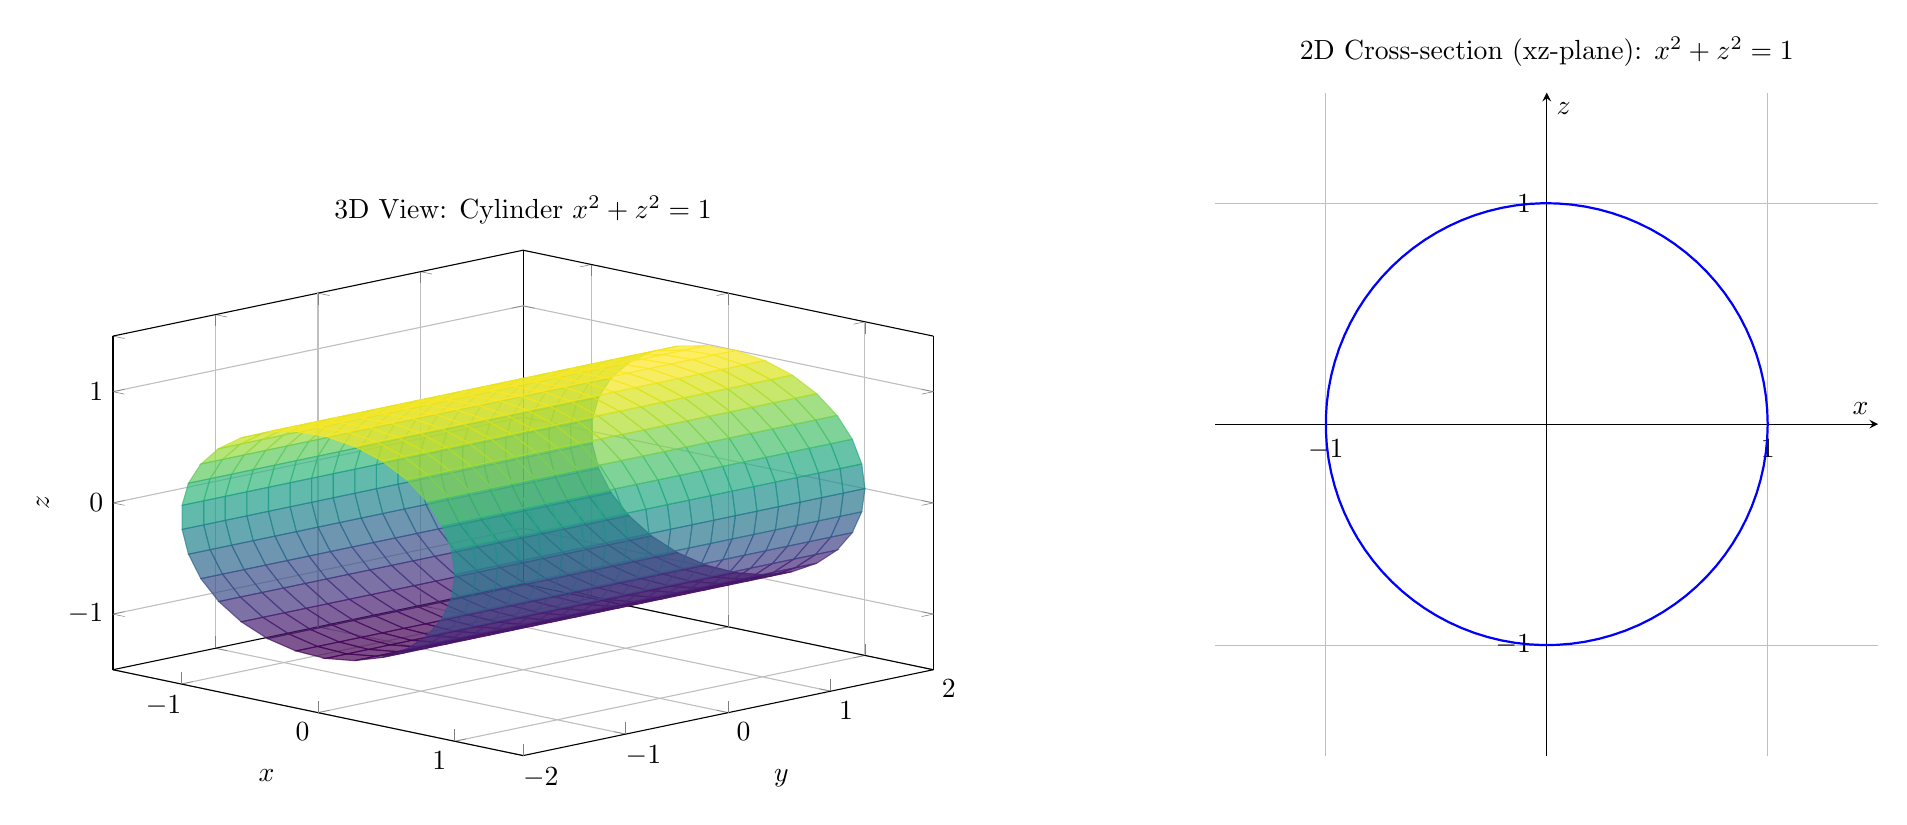
\begin{tikzpicture}

% 3D Cylinder Plot
\begin{axis}[
    view={45}{20},
    xlabel={$x$},
    ylabel={$y$},
    zlabel={$z$},
    title={3D View: Cylinder $x^2 + z^2 = 1$},
    xmin=-1.5, xmax=1.5,
    ymin=-2, ymax=2,
    zmin=-1.5, zmax=1.5,
    colormap/viridis,
    samples=30,
    samples y=20,
    domain=0:360,
    y domain=-2:2,
    grid=major,
    width=12cm,
    height=8cm
]
\addplot3[surf, shader=flat corner, opacity=0.7] 
({cos(x)}, {y}, {sin(x)});
\end{axis}

% 2D Cross-section Plot
\begin{axis}[
    shift={(14cm, 0)},
    xlabel={$x$},
    ylabel={$z$},
    title={2D Cross-section (xz-plane): $x^2 + z^2 = 1$},
    axis equal image,
    xmin=-1.5, xmax=1.5,
    ymin=-1.5, ymax=1.5,
    grid=major,
    width=10cm,
    height=10cm,
    axis lines=center,
    xtick={-1, 0, 1},
    ytick={-1, 0, 1}
]
\addplot[domain=0:360, samples=100, thick, blue] ({cos(x)}, {sin(x)});
\end{axis}

\end{tikzpicture}
\end{document}
